% DO NOT COMPILE THIS FILE DIRECTLY!
% This is included by the other .tex files.

\begin{frame}[t,plain]
\titlepage
\end{frame}

\begin{frame}[t]{Contents of this presentation}
\begin{itemize}
	\item Progress
	\item Revised backlog
	\item Second sprint description 
	\item Final sprint 
	\item Feedback
\end{itemize}
\end{frame}


\begin{frame}[t]{Progress}

\framesubtitle{Starfish: a quick recap}

\begin{itemize}
  \item System to improve knowledge sharing
  \item Network of linked (directed) documents
  \item Goal: create system that can automaticaly propose new links
\end{itemize}


\end{frame}




\begin{frame}[t]{Progress}

  \huge{Sprint One or Week Two}

\end{frame}




\begin{frame}[t]{Progress}

\framesubtitle{What did we set out to do?}

% Hier moet een afbeelding van sprint 1 backlog in

\end{frame}

\begin{frame}[t]{Progress}

\framesubtitle{What did we do?}

\begin{itemize}
\item Software skeleton
\item Nearest Neighbor
\item Different vector distance metrics
\item Document vectorizers \\
  \begin{itemize}
    \item (Weighted) tag glossary descriptor
    \item Text descriptor
    \item Tag descriptor
    \item Smoothed tag descriptor
  \end{itemize}
\item Research on other methods
\end{itemize}

\end{frame}



\begin{frame}[t]{Progress}

\framesubtitle{What didn't we do?}

\begin{itemize}
\item Automated evaluation metric
\end{itemize}

\end{frame}



\begin{frame}[t]{Progress}

\framesubtitle{Deliverable}

A program that can given a network and a new document propose new
links between the new and known documents.

\addvspace{3mm}
{\tt \$ documentlinker\\ Usage: -vectorizer <algorithm> -distance <cosine/eucledian>}

\pause
\addvspace{3mm}
Does not accept a new document yet, but will propose new documents for every
document in the data set.

\end{frame}


\begin{frame}[t]{Product Backlog}
  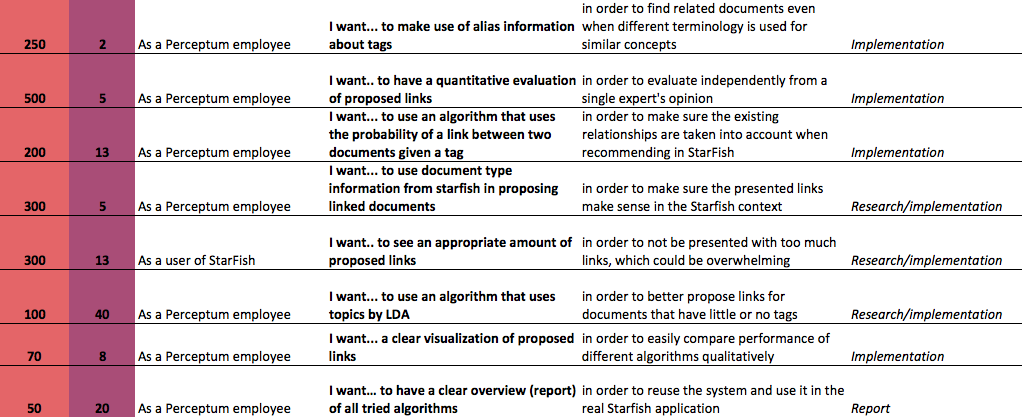
\includegraphics[width=\linewidth]{backlog2}
\end{frame}

\begin{frame}[t]{Definition of Done (recap)}
\framesubtitle{Product Backlog}

\begin{itemize}
	\item  The code is written OOP, and the classes that act correctly within the application framework
	\item The code is documented in a notebook containing examples of usage, test results and description of design choices 
	\item The code is well tested both individually as within the application flow (this may be done manually – no automated tests)
\end{itemize}
\end{frame}

\begin{frame}[t]{Sprint 2}
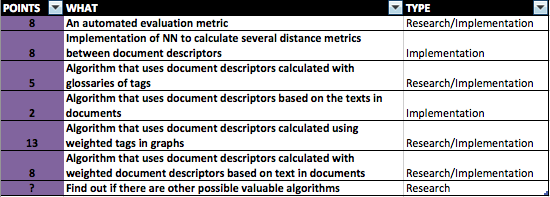
\includegraphics[width=\linewidth]{sprintt}
\end{frame}

\begin{frame}[t]{Sprint 3}

\end{frame}

\begin{frame}[t]{Feedback}
We would love to hear what you think about our planning! Are there any suggestions or questions?
\end{frame}
